\documentclass{article}
\usepackage[utf8]{inputenc}

\title{RNNs} 
\author{Sylesh Suresh and Justin Zhang}
\date{January 2018}

\usepackage{natbib}
\usepackage{graphicx}
\usepackage{epigraph}
\usepackage{float}

\begin{document}

\maketitle

\section{Introduction}
Recurrent Neural Networks (RNNs) are a type of neural network that specializes on sequential data; that is, data that is dependant on prior data. For instance, RNNs are often used for natural language processing, because a given word is more likely to appear depending on the prior words. In this vein, RNNs have been applied to tasks like machine translation, image caption generation, and word prediction. However, RNNs have also seen moderate successes in image generation and audio generation.

\section{Basic RNNs}
    In order to handle sequential data, a recurrent neural network has to be able to take in vectors of variable lengths. To do this, we design our network in the appropriate way. A RNN might look like the following:
    \begin{figure}[H]
        \centerline{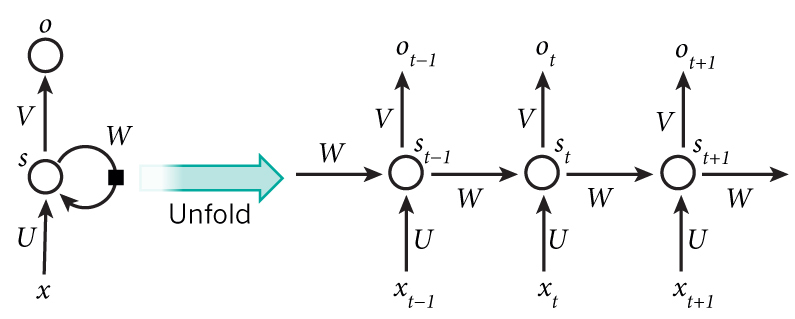
\includegraphics[scale=0.3]{rnn.jpg}}
        \caption{An unrolled RNN.}
        \label{fig:rnn}
    \end{figure}
    The figure above shows a RNN being \textit{unrolled}, that is, being written out for the entire sequence $x$. If, for example, we had a sentence composed of five words, we would have the network be unrolled into five layers, one for each word. Note that the number of layers in the network matches the length of the sequence, so we can handle variable-length vectors unlike standard feedfoward neural networks. Moreover, the hidden state $s_t$ depends on not only $x_t$ but also the state of the previous layer $s_{t-1}$, allowing RNNs to process sequential data better than feedforward networks. The output of a layer, $o_t$, is calculated from the layer's hidden state and is thus likewise reliant on the previous hidden state. Specifically, \[ s_t = f(Ux_t + Ws_{t-1})\] where U and W are weight matrices. The first hidden state $s_0$ is usually initialized to $f(Ux_0)$. The function $f$ is typically the tanh function or the ReLU function. The output $o_t$ is calculated as such: \[ o_t = softmax(Vs_t) \] where V is also a weight matrix. Note that U, V, and W are the same matrices for each layer as we are performing essentially the same operation at each time step $t$, meaning we only need to learn a few parameters. Also note that although we have an output for each layer, we may not necessarily use every one. For example, in sentiment analysis, we would only want the final output, the sentiment of the entire sentence, not the sentiment after each individual word.
    
    \subsection{Backpropagation Through Time}
     The equations for the hidden state $s_t$ and predicted output $o_t$ are:
    \[ s_t=\tanh(U x_t+W s_{t-1}) \] 
    \[ o_t= softmax(V s_t) \]
    
    \noindent Our total loss (error) function is:
    
    \begin{equation}
    \label{loss}
    L(y,\hat{y})=\sum_{t} E_t
    \end{equation}
    \noindent This is simply the sum of the losses at each time step. We can define the loss at each time step as:
    \begin{equation}
    \label{oneloss}
    E_t=-y_t\log o_t.
    \end{equation}
    \noindent where $y_t$ is the ground truth at a particular time step $t$.
    \noindent Note that the loss functions are dot products between the vectors $y_t$ and the resulting vector of the element-wise logarithm of $o_t$. 
    \noindent The weight matrices to be trained are $U$, $V$, and $W$. For $V$, by the chain rule, we find:
    \[ \frac{\partial E_t}{\partial V} = \frac{\partial E_t}{\partial o_t}\frac{\partial o_t}{\partial (V s_t)}\frac{\partial (V s_t)}{\partial V} \]
    From this, we can derive:
    \[ \frac{\partial E_t}{\partial V} = (o_t - y_t) \times s_t \]
    Where $\times$ is the cross product.
    For $W$, we can similarly apply the chain rule:
    \[ \frac{\partial E_t}{\partial W} = \frac{\partial E_t}{\partial o_t}\frac{\partial o_t}{\partial s_t}\frac{\partial s_t}{\partial W} \]
    We can use the chain rule on the $\frac{\partial s_t}{\partial W}$ term again as $s_t$ depends on $s_{t-1}$ and we find:
    \[ \frac{\partial E_t}{\partial W} = \frac{\partial E_t}{\partial o_t}\frac{\partial o_t}{\partial s_t}\sum_{i=0}^t \frac{\partial s_t}{\partial s_i}\frac{\partial s_i}{\partial W} \]
    From this, we can derive:
    \[ \frac{\partial E_t}{\partial W} = (o_t - y_t)V\sum_{i=0}^t \frac{\partial s_t}{\partial s_i}\frac{\partial s_i}{\partial W} \]
    The partial derivative with respect to $U$ is essentially identical:
     \[ \frac{\partial E_t}{\partial U} = (o_t - y_t)V\sum_{i=0}^t \frac{\partial s_t}{\partial s_i}\frac{\partial s_i}{\partial U} \]   
    \subsection{Problems with Long-term Dependency}
    The $\sum_{i=0}^t \frac{\partial s_t}{\partial s_i}\frac{\partial s_i}{\partial W}$ term causes the vanishing gradient problem, which means that the network tends to forget words over time, which can prove troublesome. Let's take a word predictor, for instance. Given part of a sentence, predict the next word. This structure would work quite well for a sentence like "I ate some delicious ice \_\_\_\_"; "ice" provides a significant cue that the next word might be "cream." However, given a sentence like "I went to the ice cream store, but I forgot to bring my \_\_\_\_", it will likely have trouble guessing "wallet." 

    This is the problem of long-term dependencies; the network will "forget" words over time. We can remedy this issue with other types of RNNs such as LSTMs, which we will cover later on.
\section{Types of RNNs}
    \begin{figure}[H]
        \centerline{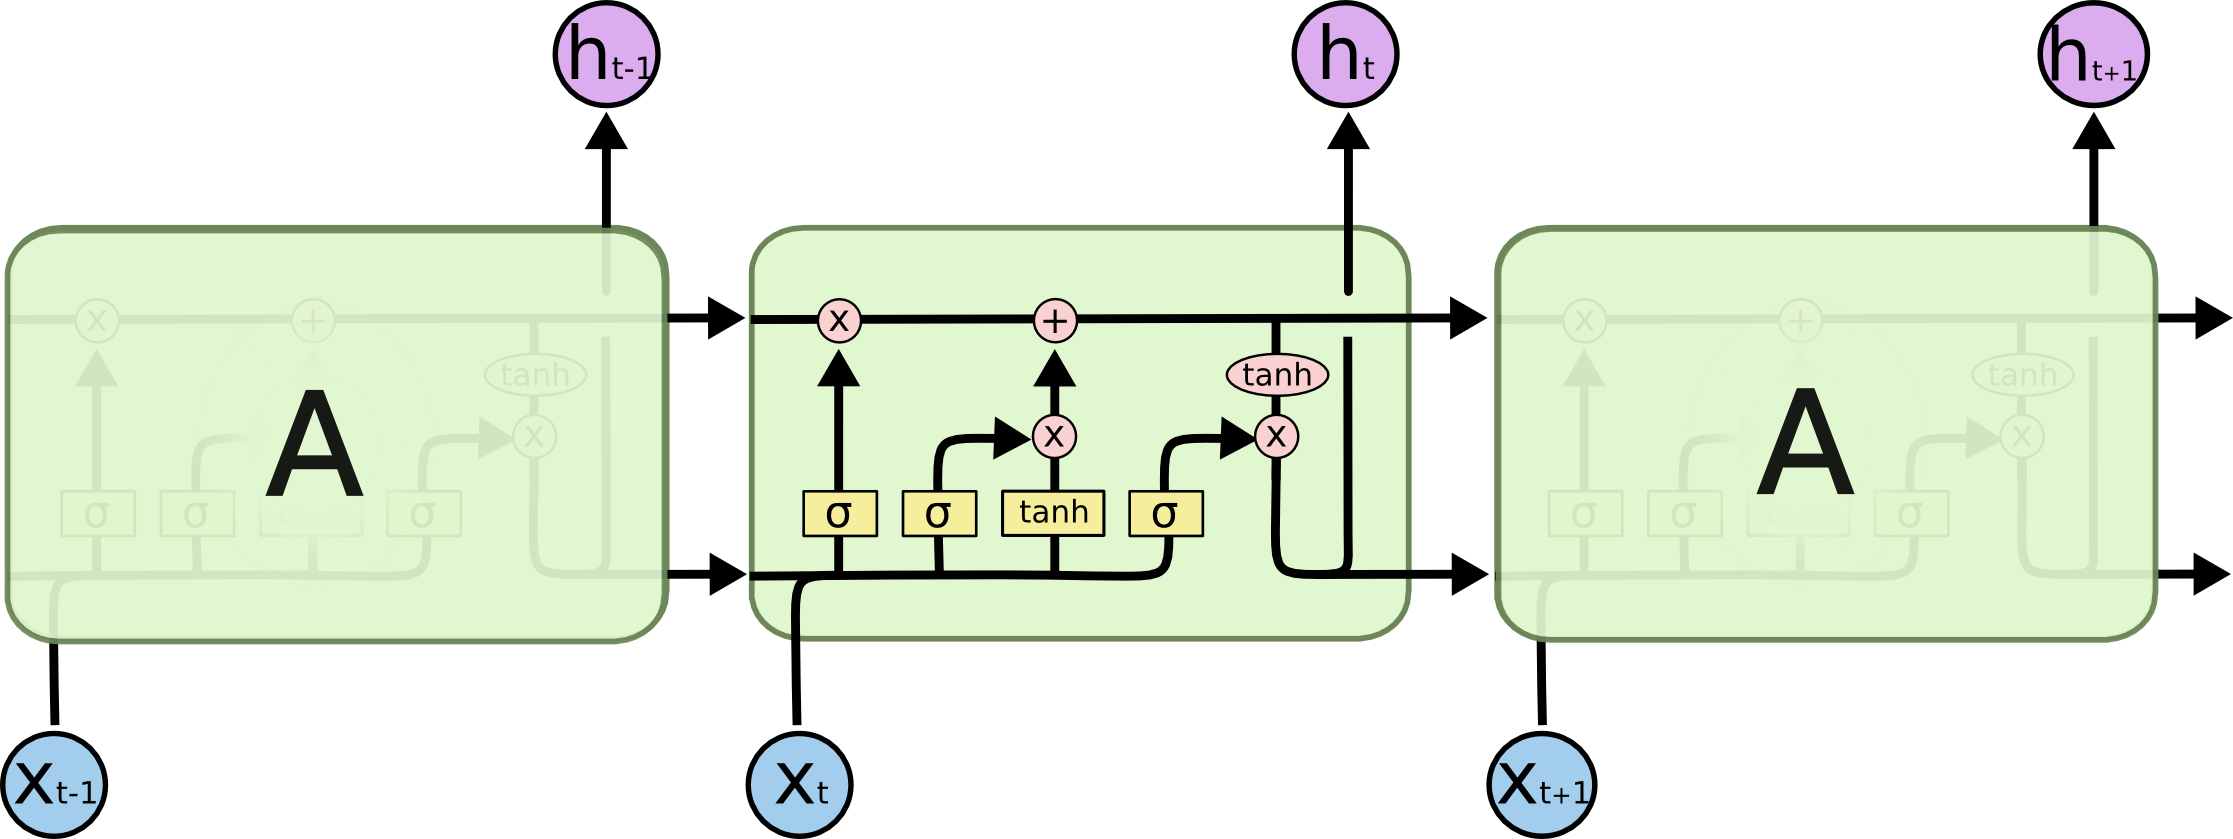
\includegraphics[scale=0.4]{LSTM.png}}
        \caption{An LSTM cell.}
        \label{fig:lstm}
    \end{figure}
    An Long Short Term Memory network (LSTM) attempts to alleviate this issue by having a "forget gate," which allows the network to select parts of an input vector to "remember" (i.e. pass on to the next cell) or "forget." It additionally has a mechanism to store and update the cell state. Let's walk through the cell step-by-step.
    \subsection{LSTM walk-through}
    \begin{figure}[H]
        \centerline{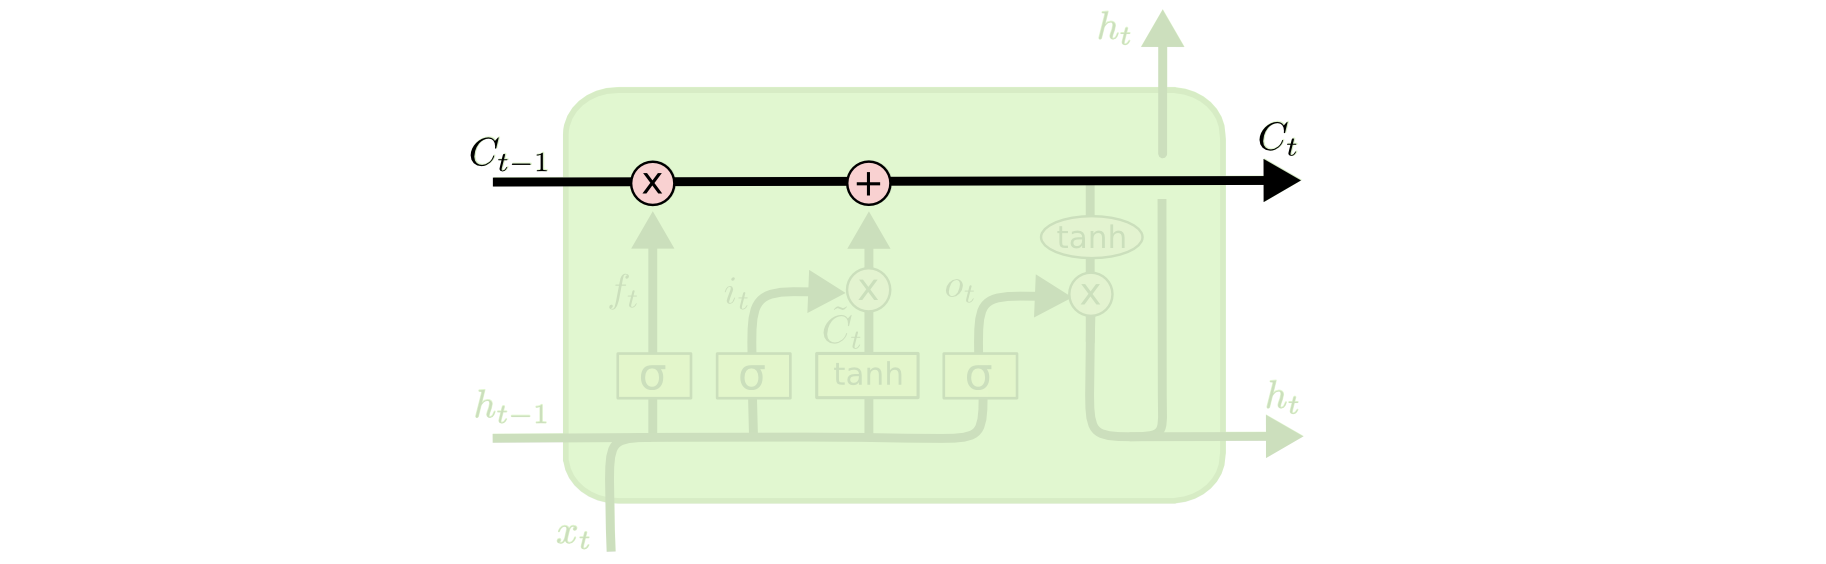
\includegraphics[scale=0.4]{LSTM0.png}}
        \caption{Cell state.}
        \label{fig:lstm0}
    \end{figure}
    First off, the cell state. This is the pathway in which information flows from cell-to-cell. It was designed so that this would have little interaction, so as to store long-term data with little change. 
    
    \begin{figure}[H]
        \centerline{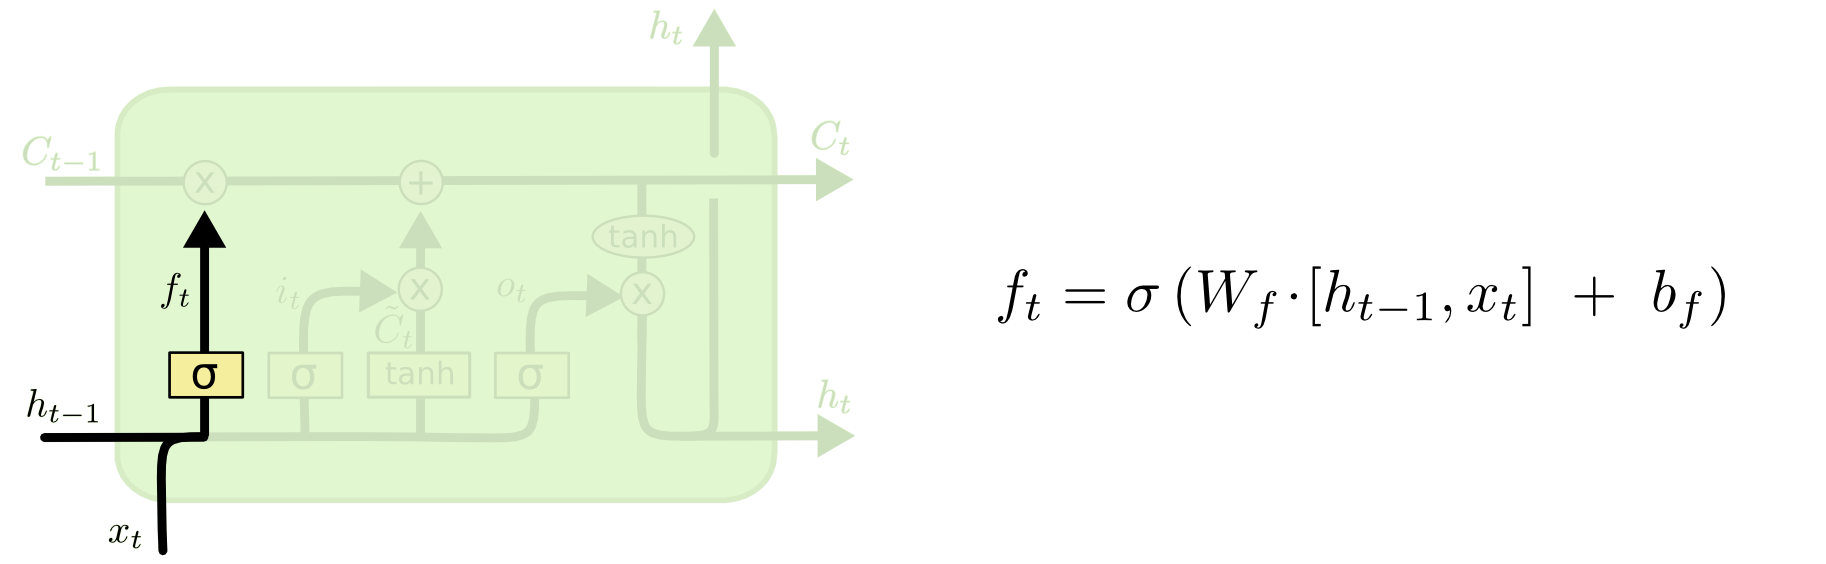
\includegraphics[scale=0.4]{LSTM1.png}}
        \caption{The forget gate.}
        \label{fig:lstm1}
    \end{figure}
    This is the forget gate. We use a sigmoid activation conditioned on the input and prior output, which gives us outputs between $0$ and $1$. Since we're multiplying this value to the cell state, an output of $0$ would correspond to completely forgetting everything, $1$ remembering everything. This is done so as to update old information with more the more recent context.
    
    \begin{figure}[H]
        \centerline{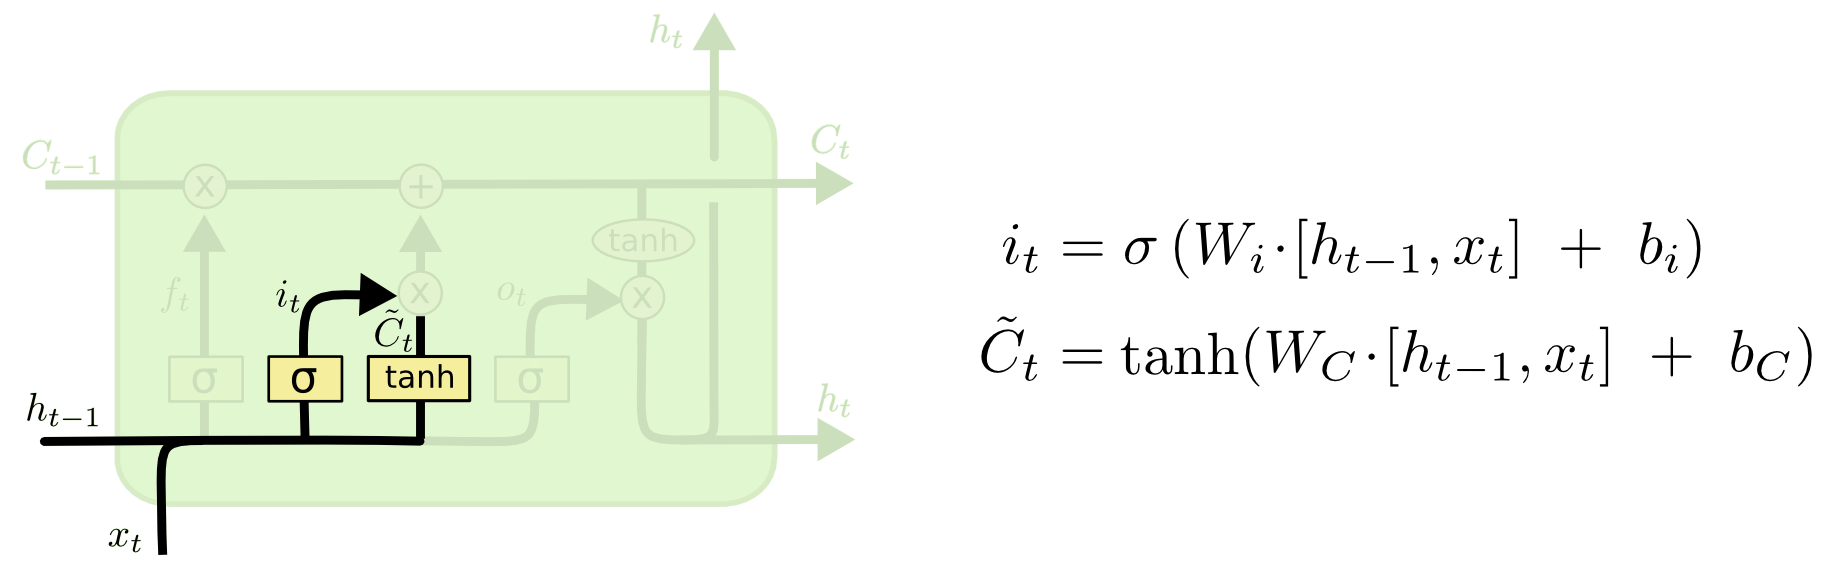
\includegraphics[scale=0.4]{LSTM2.png}}
        \caption{Updating the cell state.}
        \label{fig:lstm2}
    \end{figure}
    \begin{figure}[H]
        \centerline{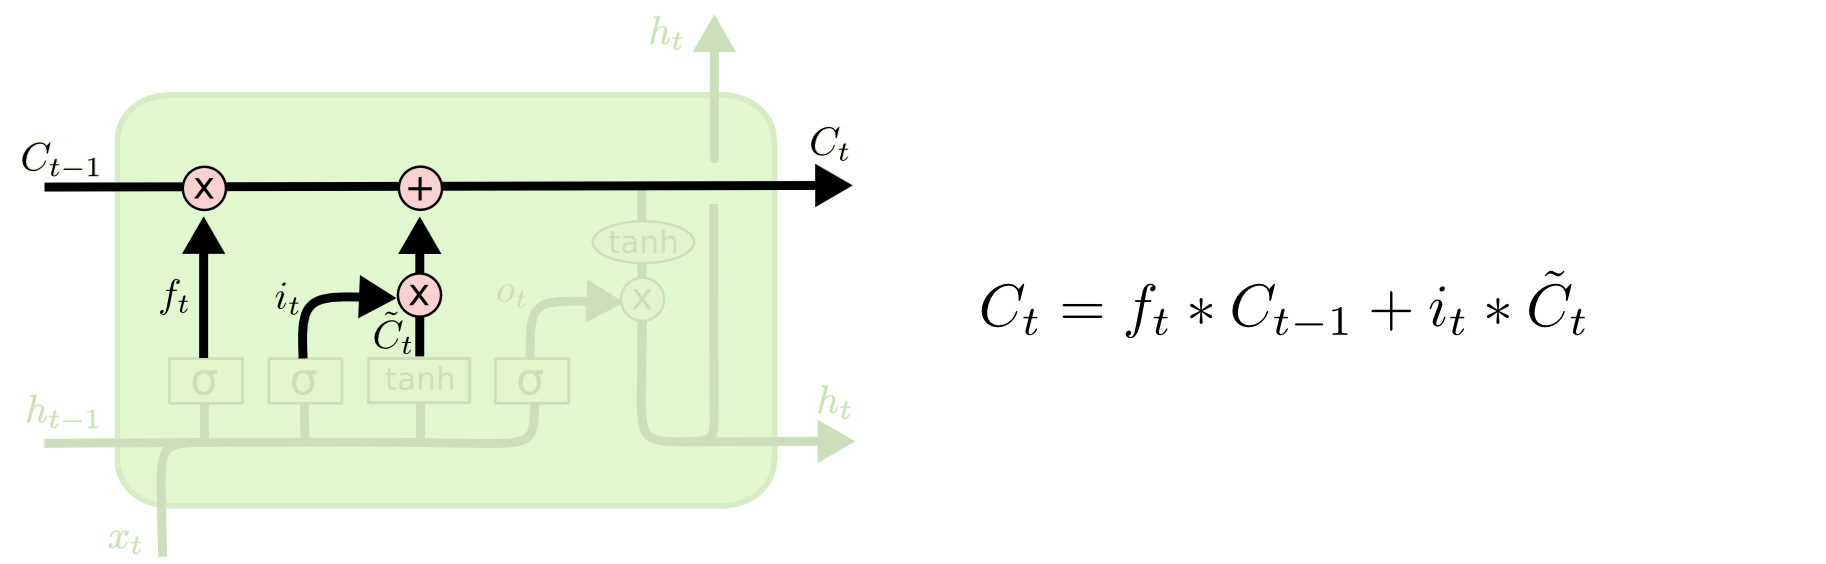
\includegraphics[scale=0.4]{LSTM3.png}}
        \caption{Outputting the cell state.}
        \label{fig:lstm3}
    \end{figure}
    Next, we add a vector to the cell state based on the input and previous output, so as to update the state. Note that we're adding values between $-1$ and $1$; $\tanh$ outputs $-1$ to $1$, and the sigmoid outputs $0$ to $1$, which determines the magnitude of the update. 
    \begin{figure}[H]
        \centerline{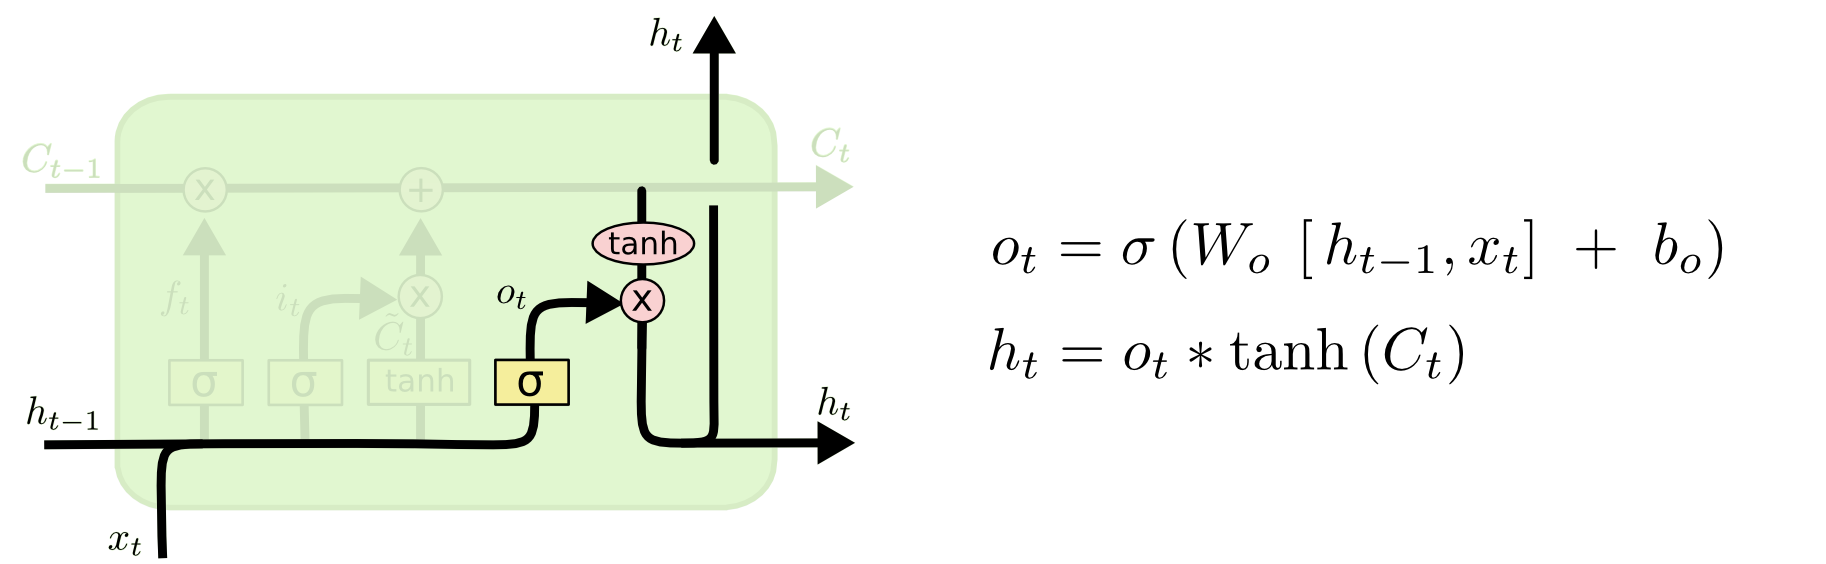
\includegraphics[scale=0.4]{LSTM4.png}}
        \caption{Outputting the final value.}
        \label{fig:lstm4}
    \end{figure}
    Lastly, we want to output $h_i$. This is determined by the cell state, which is run through $\tanh$ to bound the values between $-1$ and $1$. The sigmoid, whose output is conditioned on the previous cell output and current input, allows the cell to select which parts of the cell state to output (the sigmoid will output $0$ for the parts it does not want to output, and vice-versa). 
    
    Then, the process repeats, with the next input.
    \subsection{GRUs}
        
        \begin{figure}[H]
            \centerline{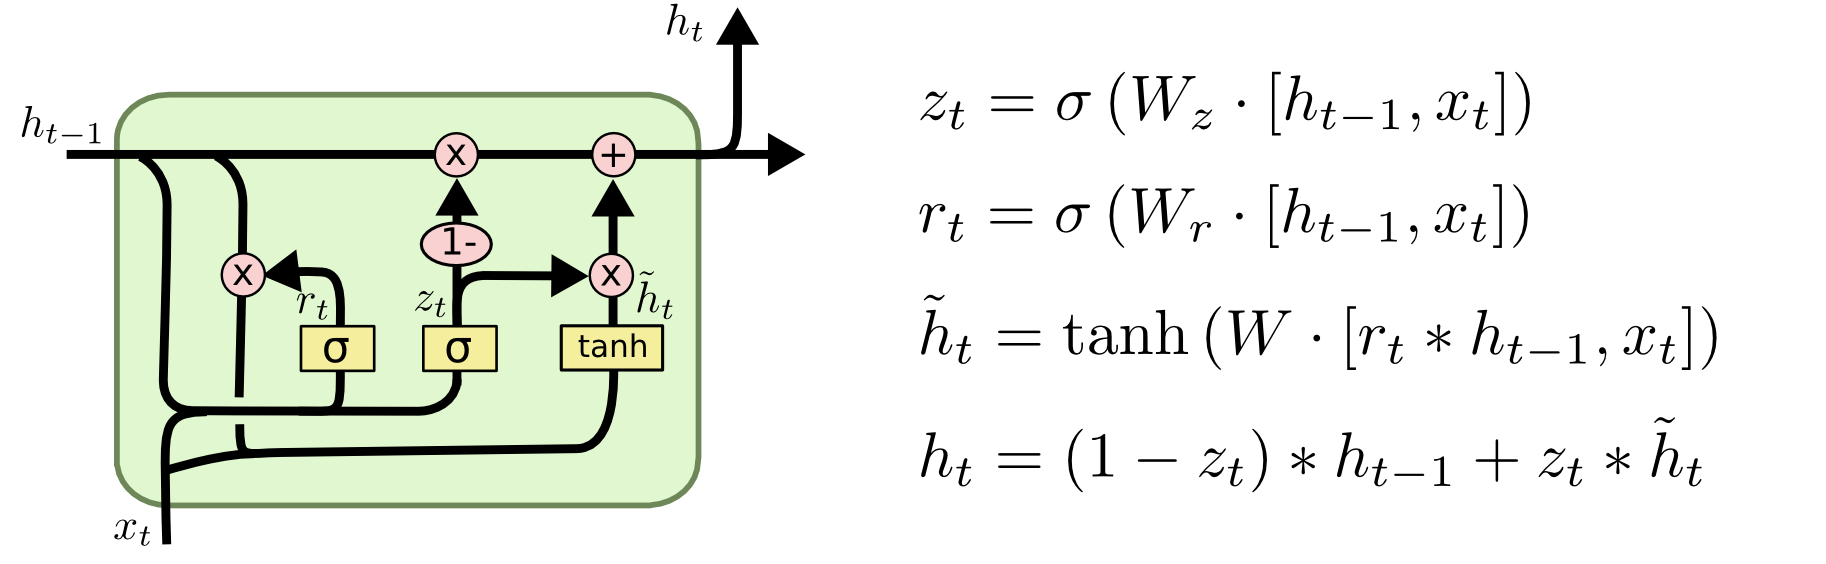
\includegraphics[scale=0.4]{GRU.png}}
            \caption{A GRU cell.}
            \label{fig:gru}
        \end{figure}
        A Gated Recurrent Unit (GRU) is an alternative to an LSTM that is computationally simpler. It opts to combine the update and forget mechanisms into an "update" mechanism, and also combines the hidden state and the cell state. GRUs are becoming increasingly popular as the perform as well as LSTMs on some tasks at a significantly lower computational cost.
\section{Conclusion}
    There are many other types of RNNs; LSTMs and GRUs are two of the most popular. Additionally, there have been advancements on RNNs themselves; "attention" mechanisms are popular in tasks such as machine translation and caption generation. 
    
    For NLP tasks, we recommend investigating word vectors (Word2Vec, skip-thought vectors, etc.) to encode words to vectors. Also, using RNNs as the basis for an encoder/decoder model is widely used to translate sequences (e.g. machine translation). We encourage you to further investigate these areas!
    
\end{document}
